% Figure 2 of the manuscript: the three regimes of a dissipative system.
% Compile with: pdflatex fig-regimes.tex
\documentclass[12pt,border=2pt]{standalone}
\usepackage{amsmath,amssymb}
\usepackage{tikz}
\begin{document}
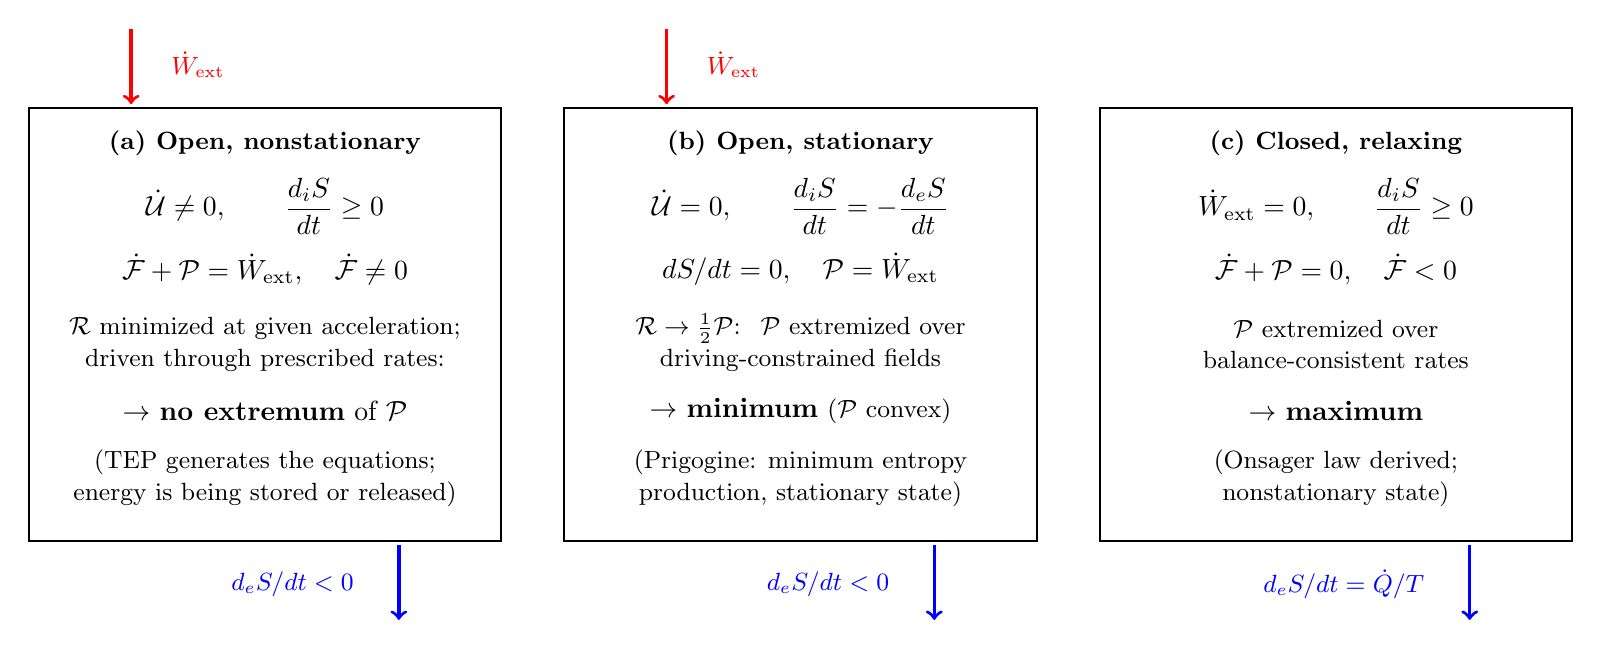
\begin{tikzpicture}
% ===== (a) open system, nonstationary =====
\begin{scope}[xshift=0cm]
\draw[thick] (-3.0, -2.75) rectangle (3.0, 2.75);
\node at (0, 2.3) {\small\bfseries (a) Open, nonstationary};
\node at (0, 1.5) {$\dot{\mathcal{U}} \neq 0, \qquad \dfrac{d_i S}{dt} \geq 0$};
\node at (0, 0.7) {$\dot{\mathcal{F}} + \mathcal{P} = \dot{W}_{\text{ext}}, \quad \dot{\mathcal{F}} \neq 0$};
\node at (0, -0.05) {\small $\mathcal{R}$ minimized at given acceleration;};
\node at (0, -0.45) {\small driven through prescribed rates:};
\node at (0, -1.1) {$\to$ \textbf{no extremum} of $\mathcal{P}$};
\node at (0, -1.75) {\small (TEP generates the equations;};
\node at (0, -2.15) {\small energy is being stored or released)};
\draw[->, very thick, red] (-1.7, 3.75) -- (-1.7, 2.8);
\node[red] at (-0.85, 3.3) {\small $\dot{W}_{\text{ext}}$};
\draw[->, very thick, blue] (1.7, -2.8) -- (1.7, -3.75);
\node[blue] at (0.35, -3.3) {\small $d_e S/dt < 0$};
\end{scope}
% ===== (b) open system, stationary state =====
\begin{scope}[xshift=6.8cm]
\draw[thick] (-3.0, -2.75) rectangle (3.0, 2.75);
\node at (0, 2.3) {\small\bfseries (b) Open, stationary};
\node at (0, 1.5) {$\dot{\mathcal{U}} = 0, \qquad \dfrac{d_i S}{dt} = -\dfrac{d_e S}{dt}$};
\node at (0, 0.7) {$dS/dt = 0, \quad \mathcal{P} = \dot{W}_{\text{ext}}$};
\node at (0, -0.05) {\small $\mathcal{R} \to \tfrac{1}{2}\mathcal{P}$: \ $\mathcal{P}$ extremized over};
\node at (0, -0.45) {\small driving-constrained fields};
\node at (0, -1.1) {$\to$ \textbf{minimum} \small($\mathcal{P}$ convex)};
\node at (0, -1.75) {\small (Prigogine: minimum entropy};
\node at (0, -2.15) {\small production, stationary state)};
\draw[->, very thick, red] (-1.7, 3.75) -- (-1.7, 2.8);
\node[red] at (-0.85, 3.3) {\small $\dot{W}_{\text{ext}}$};
\draw[->, very thick, blue] (1.7, -2.8) -- (1.7, -3.75);
\node[blue] at (0.35, -3.3) {\small $d_e S/dt < 0$};
\end{scope}
% ===== (c) closed system, relaxing =====
\begin{scope}[xshift=13.6cm]
\draw[thick] (-3.0, -2.75) rectangle (3.0, 2.75);
\node at (0, 2.3) {\small\bfseries (c) Closed, relaxing};
\node at (0, 1.5) {$\dot{W}_{\text{ext}} = 0, \qquad \dfrac{d_i S}{dt} \geq 0$};
\node at (0, 0.7) {$\dot{\mathcal{F}} + \mathcal{P} = 0, \quad \dot{\mathcal{F}} < 0$};
\node at (0, -0.05) {\small $\mathcal{P}$ extremized over};
\node at (0, -0.45) {\small balance-consistent rates};
\node at (0, -1.1) {$\to$ \textbf{maximum}};
\node at (0, -1.75) {\small (Onsager law derived;};
\node at (0, -2.15) {\small nonstationary state)};
\draw[->, very thick, blue] (1.7, -2.8) -- (1.7, -3.75);
\node[blue] at (0.1, -3.3) {\small $d_e S/dt = \dot{Q}/T$};
\end{scope}
\end{tikzpicture}}
\end{document}
